
%version 2: \usepackage{hyperref}


%%%%%%%%%%%%%%%%%%%%%%%%%%%%%%%%%%%%%%%%%%%%%%%%%%%%%%%%%%%%%%%%%%%%%%%%
%Para las ecuaciones siempre es Ec.(n).
%Para las figuras siempre es Fig.n, incluso en el caption de la figura. Tambien las Tablas
%Para las referencias es [n]
%%%%%%%%%%%%%%%%%%%%%%%%%%%%%%%%%%%%%%%%%%%%%%%%%%%%%%%%%%%%%%%%%%%%%%%%

\documentclass[
reprint,
%notitlepage,
%superscriptaddress,
%groupedaddress,
%unsortedaddress,
%runinaddress,
%frontmatterverbose, 
%preprint,
%showpacs,preprintnumbers,
%nofootinbib,
%nobibnotes,
%bibnotes,
%11 pt,
amsmath,
amssymb,
aps,
pra,
%prb,
%rmp,
%tightenlines %esto hizo el milagro de sacar los espacios en blancos estocásticos (?)
%prstab,
%prstper,
%floatfix,\textbf{}
]{revtex4-1} %Instalar primero para usarlo. Paquete malo.

%\documentclass[onecolumn, aps, amsmath,amssymb ]{article}
\usepackage{lipsum}  
\usepackage{graphicx}% Include figure files
\usepackage{subfig}
\usepackage{braket}
\usepackage{comment} %comment large chunks of text
\usepackage{dcolumn}% Align table columns on decimal point
\usepackage{bm}% bold math
%\usepackage{hyperref}% add hypertext capabilities
\usepackage[mathlines]{lineno}% Enable numbering of text and display math
%\linenumbers\relax % Commence numbering lines
\usepackage{mathtools} %% Para el supraíndice

\usepackage[nice]{nicefrac}

%%%%%%%El Señor Español%%%%%%%%%%%%%%%%%%%%%%%%%%%
\usepackage[utf8]{inputenc} %acento
\usepackage[
spanish, %El lenguaje.
es-tabla, %La tabla y no cuadro.
activeacute, %El acento.
es-nodecimaldot %Punto y no coma con separador de números
]{babel}
\usepackage{microtype} %para hacerlo más bonito :33 como vos (?) 
%%%%%%%%%%%%%%%%%%%%%%%%%%%%%%%%%%%%%%%%%%%%%%%%%%%
%%%%%%%%% Para que las imágenes se queden dónde las quiero (?
\usepackage{float}
%%%%%%%%%%

\usepackage{hyperref} % Para usar \url

%%%%%%%%Cambia a Fig de Figure%%%%%%%%%%
\makeatletter
\renewcommand{\fnum@figure}{Fig. \thefigure} 
\makeatother
%%%%%%%%%%%%%%%%%%%%%%%%%%%%%%%%%%%%%%%%
\raggedbottom

\usepackage{physics}
\begin{document}
%%%%%%%%%%%%%%%%%%%%%%%%%%%%%%%%%%Título%%%%%%%%%%%%%%%%%%%%%%%%%%%%%%%%%%%%%%
%%%%%%%%%%%%%%%%%%%%%%%%%%%%%%%%%%%%%%%%%%%%%%%%%%%%%%%%%%%%%%%%%%%%%%%%%%%%%%

\title{Reporte de Septiembre (arrastrando Agosto)}
\author{Evelyn~G.~Coronel}

\affiliation{
Tesis de Maestría en Ciencias Físicas\\ Instituto Balseiro\\}

\date[]{\lowercase{1 de octubre de 2020}} %%lw para lw, [] sin date


\maketitle
%\onecolumngrid

\section*{Bineado}

Para verificar que mi código funciona bien, hice la clasificación de los eventos del Main Array y de All Triggers, sólo cambiando la línea donde se lee el archivo de eventos.  En la Fig.\ref{fig:Bineado} se consideran los eventos $6T5$ por encima de $3\,EeV$ desde el $1\/1\/2014$  hasta el $31\/12\/2019$. Se observa que la cantidad de eventos en el Main Array tiene una variación del $2.5\%$ con una tendencia en aumentar con $\sin^2 \theta$. En cambio para todos All Triggers existe una variación de  $\sim 10 \%$.

\begin{table}[H]
    \begin{small}
        \begin{center}
            \begin{tabular}[c]{c|c|c|c}
                bin & $\sin^2\theta$ & All Triggers & Main Array \\
                \hline
                1& 0.00-0.15 & 19605 & 15133\\
                2& 0.15-0.30 & 18489 & 15385\\
                3& 0.30-0.45 & 17863 & 15488\\
                4& 0.45-0.60 & 19390 & 15695\\
                5& 0.60-0.75 & 21440 & 15853\\
            \end{tabular}            \caption{}
        \label{tab:}
    \end{center}
    \end{small}
\end{table}

\begin{figure}[H]
    \begin{small}
        \begin{center}
            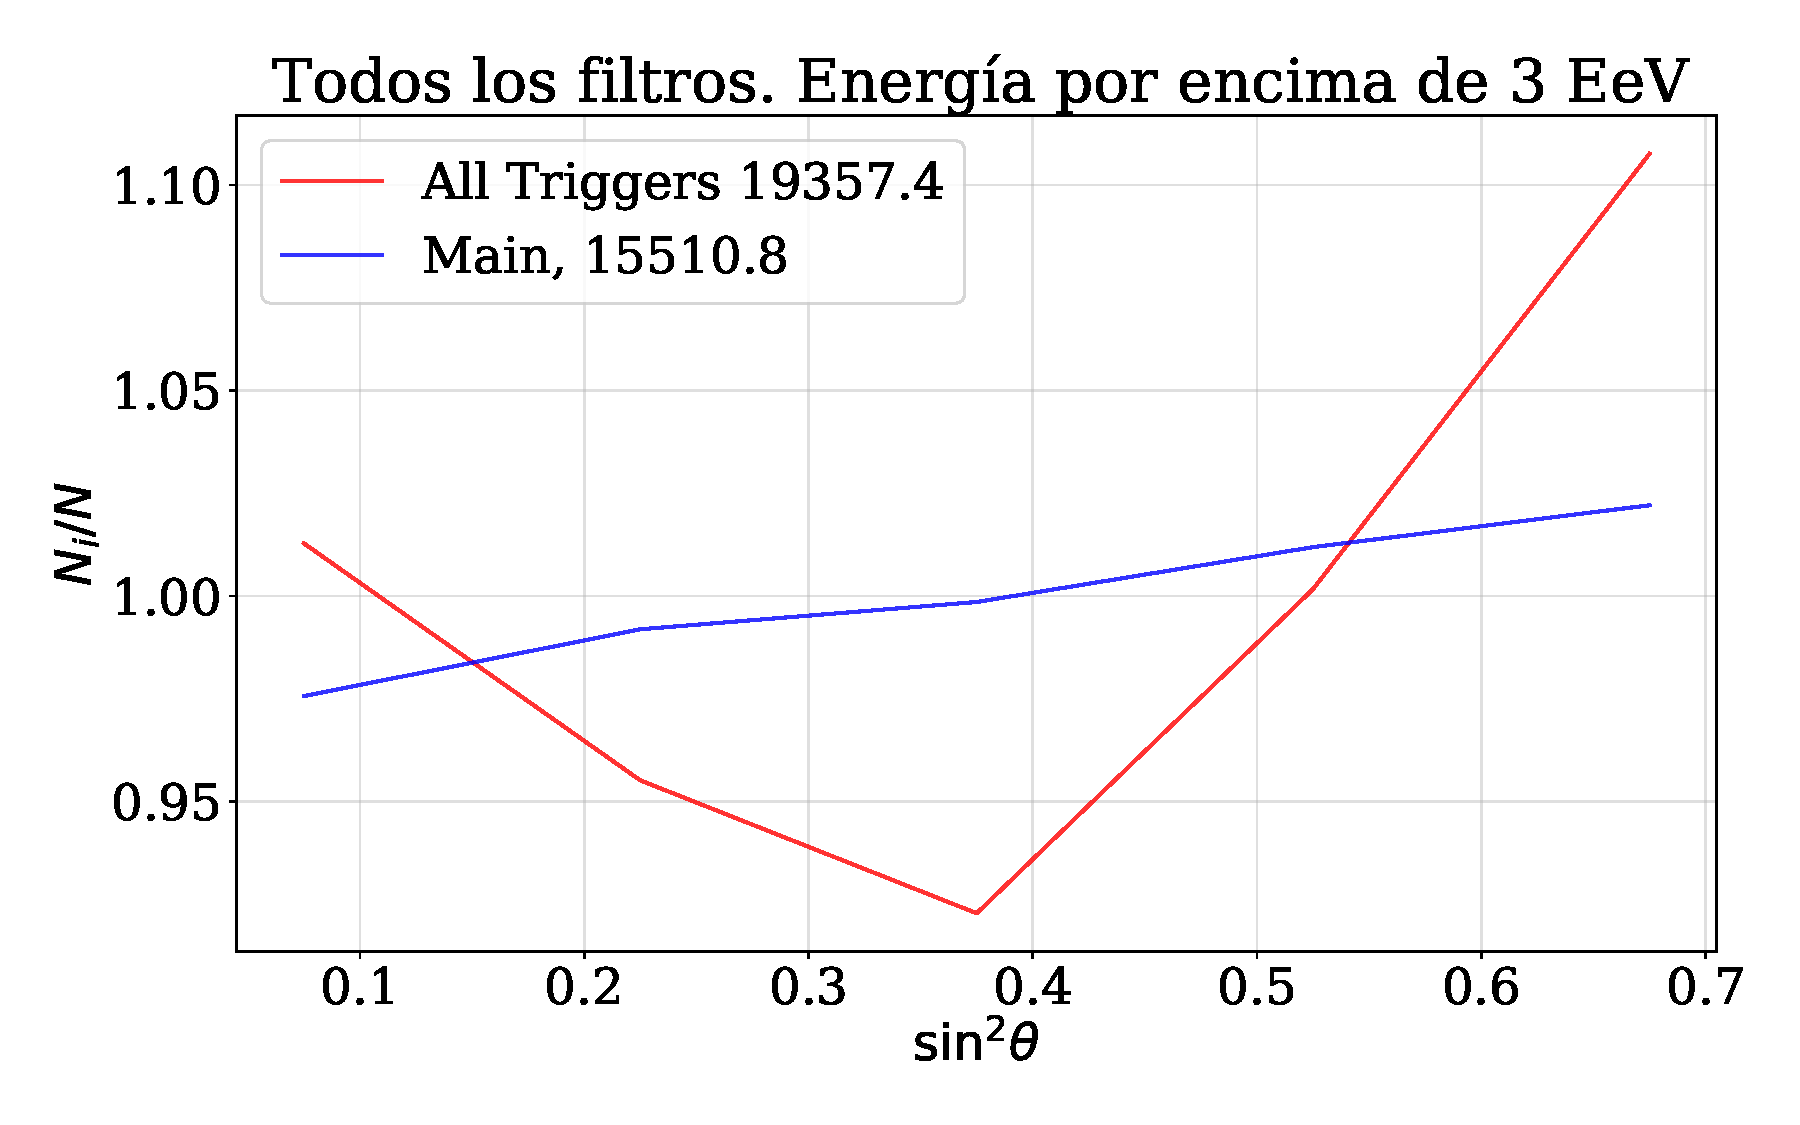
\includegraphics[width=0.45\textwidth]{eventos_bin_sin_theta.pdf}
        \end{center}
        \caption{Bineado de eventos por $\sin^2\theta$}
        \label{fig:Bineado}
    \end{small}
\end{figure}


\section*{Tabla para distintos rangos}
\begin{table}[H]
    \begin{small}
        \begin{center}
            \begin{tabular}[c]{c|l|c}
                \multicolumn{1}{c|}{\textbf{Rango [EeV]}} & 
                \multicolumn{1}{c|}{\textbf{Eventos}} 
                & \bf{Energía Media} \\
                \hline
                0.25 - 0.5 & $4\,334\,500$ & 0.374\\
                0.5 - 1 &   $3\,846\,087$ & 0.687\\
                1   - 2 & $1\,141\,168$ & 1.315 \\
            \end{tabular}
            \caption{Tabla de eventos por rango de energía \footnote{Energía según el archivo del Herald}}
            \label{tab:}
        \end{center}
    \end{small}
\end{table}

\section*{Reconstrucción de eventos con los parámetros del clima}


Para obtener los nuevos parámetros del clima, considero el conjunto de datos filtrado mediante el valor de $S_{38}=5.36\,$VEM sin la corrección de clima de la colaboración. Es es posible debido a que el archivo del Herald tiene los valores de $S(1000)$ sin corregir (columna 12) y los corregidos (columna 37), por lo tanto $S_{38}= S_{38,w}\nicefrac{S(1000)}{S(1000)_w} = \$12*\$47/\$37$. Este valor de $S_{38}$ de referencia corresponde aproximadamente a la energía de un evento 1 EeV. Considerando lo que había hecho durante la licenciatura, tenemos que:
\begin{align}
    S &= S_0 (1 + \alpha_P..+ \alpha_\rho*... + \beta_\rho...)\\
    \dv{R}{sin^2\theta} &=  R_0 \big[ 1 + a_P.. + a_\rho ..+ b_\rho..  \big]
\end{align}
donde $S$ es la señal medida, $S_0$ la señal esperada, $\nicefrac{dR}{d(sin^\theta)}$ es la tasa de eventos por ángulo sólido, $R_0$ la tasa media y  $a_P = 2.363 \alpha_P$, también  los otros parámetros.

Los parámetros $a_P$, $b_\rho$ y $a_\rho$ en función de $\sin^2 \theta$ son utilizados para ajustar un polinomio de orden 2. Así mediante el  valor de $\theta$ asociado a un evento, podemos tener los parámetros del clima para corregir ese evento.

\begin{figure}[H]
    \begin{small}
        \begin{center}
            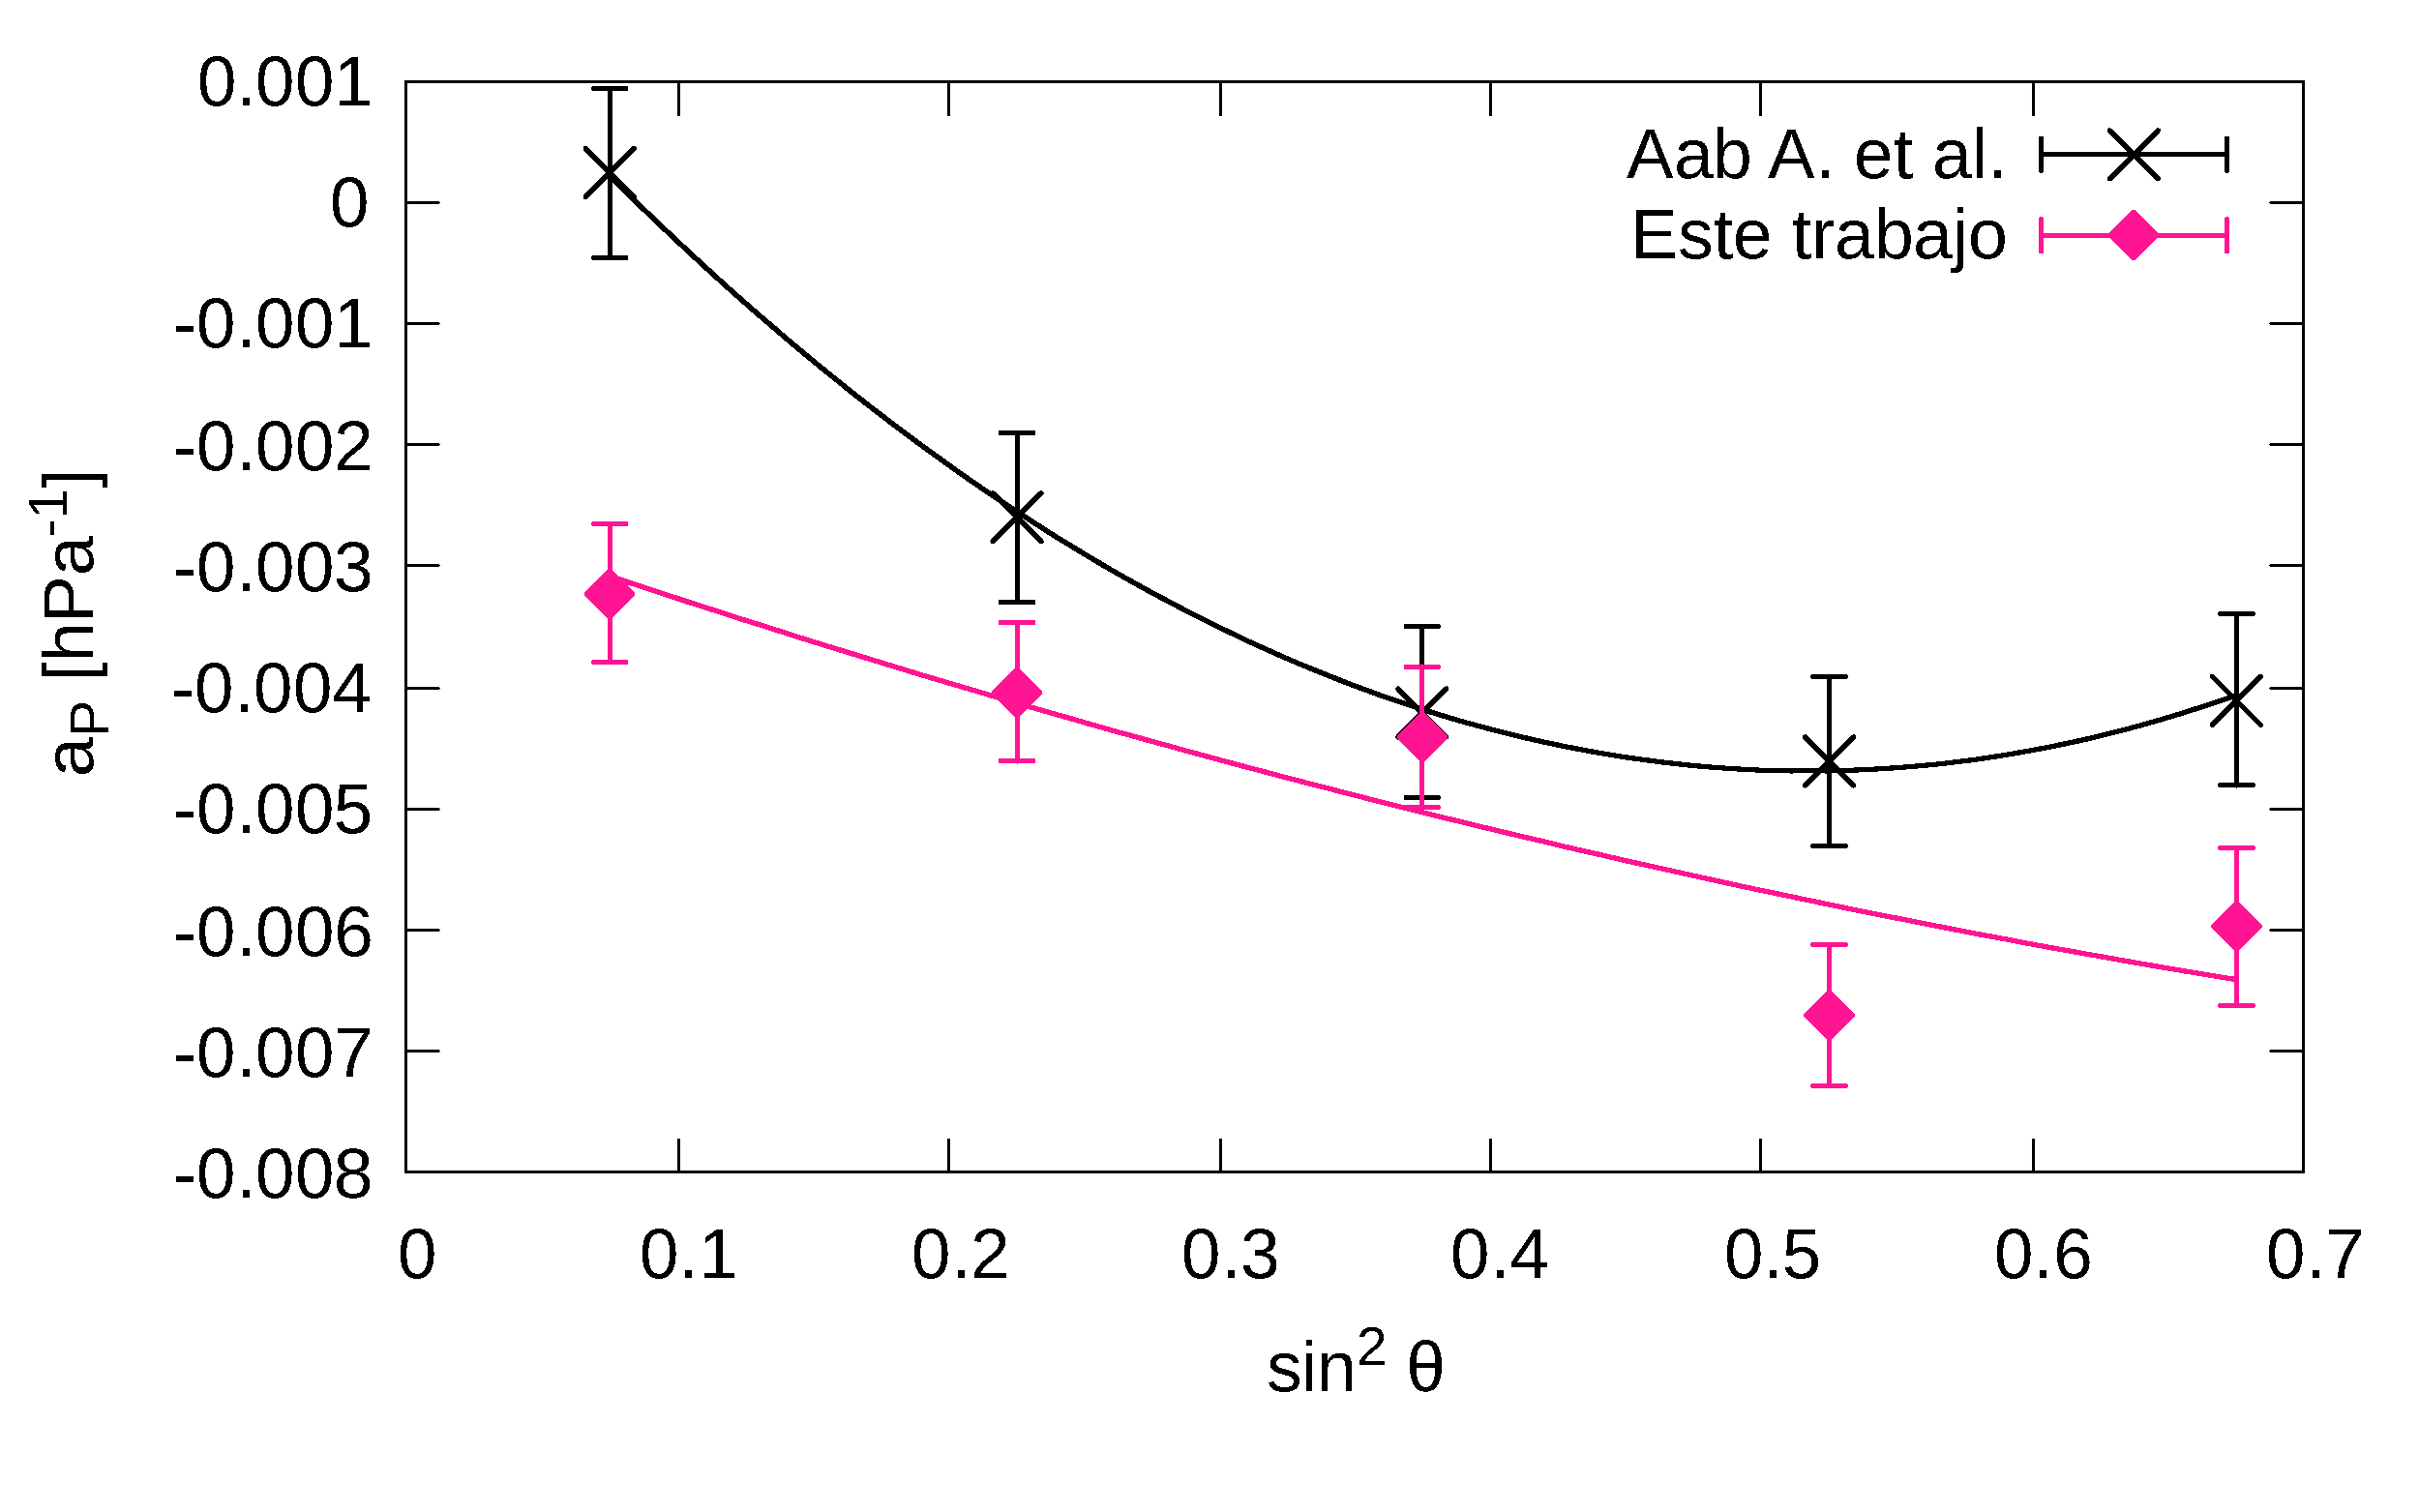
\includegraphics[width=0.5\textwidth]{ap.pdf}
        \end{center}
        \caption{}
        \label{fig:}
    \end{small}
\end{figure}


\begin{figure}[H]
    \begin{small}
        \begin{center}
            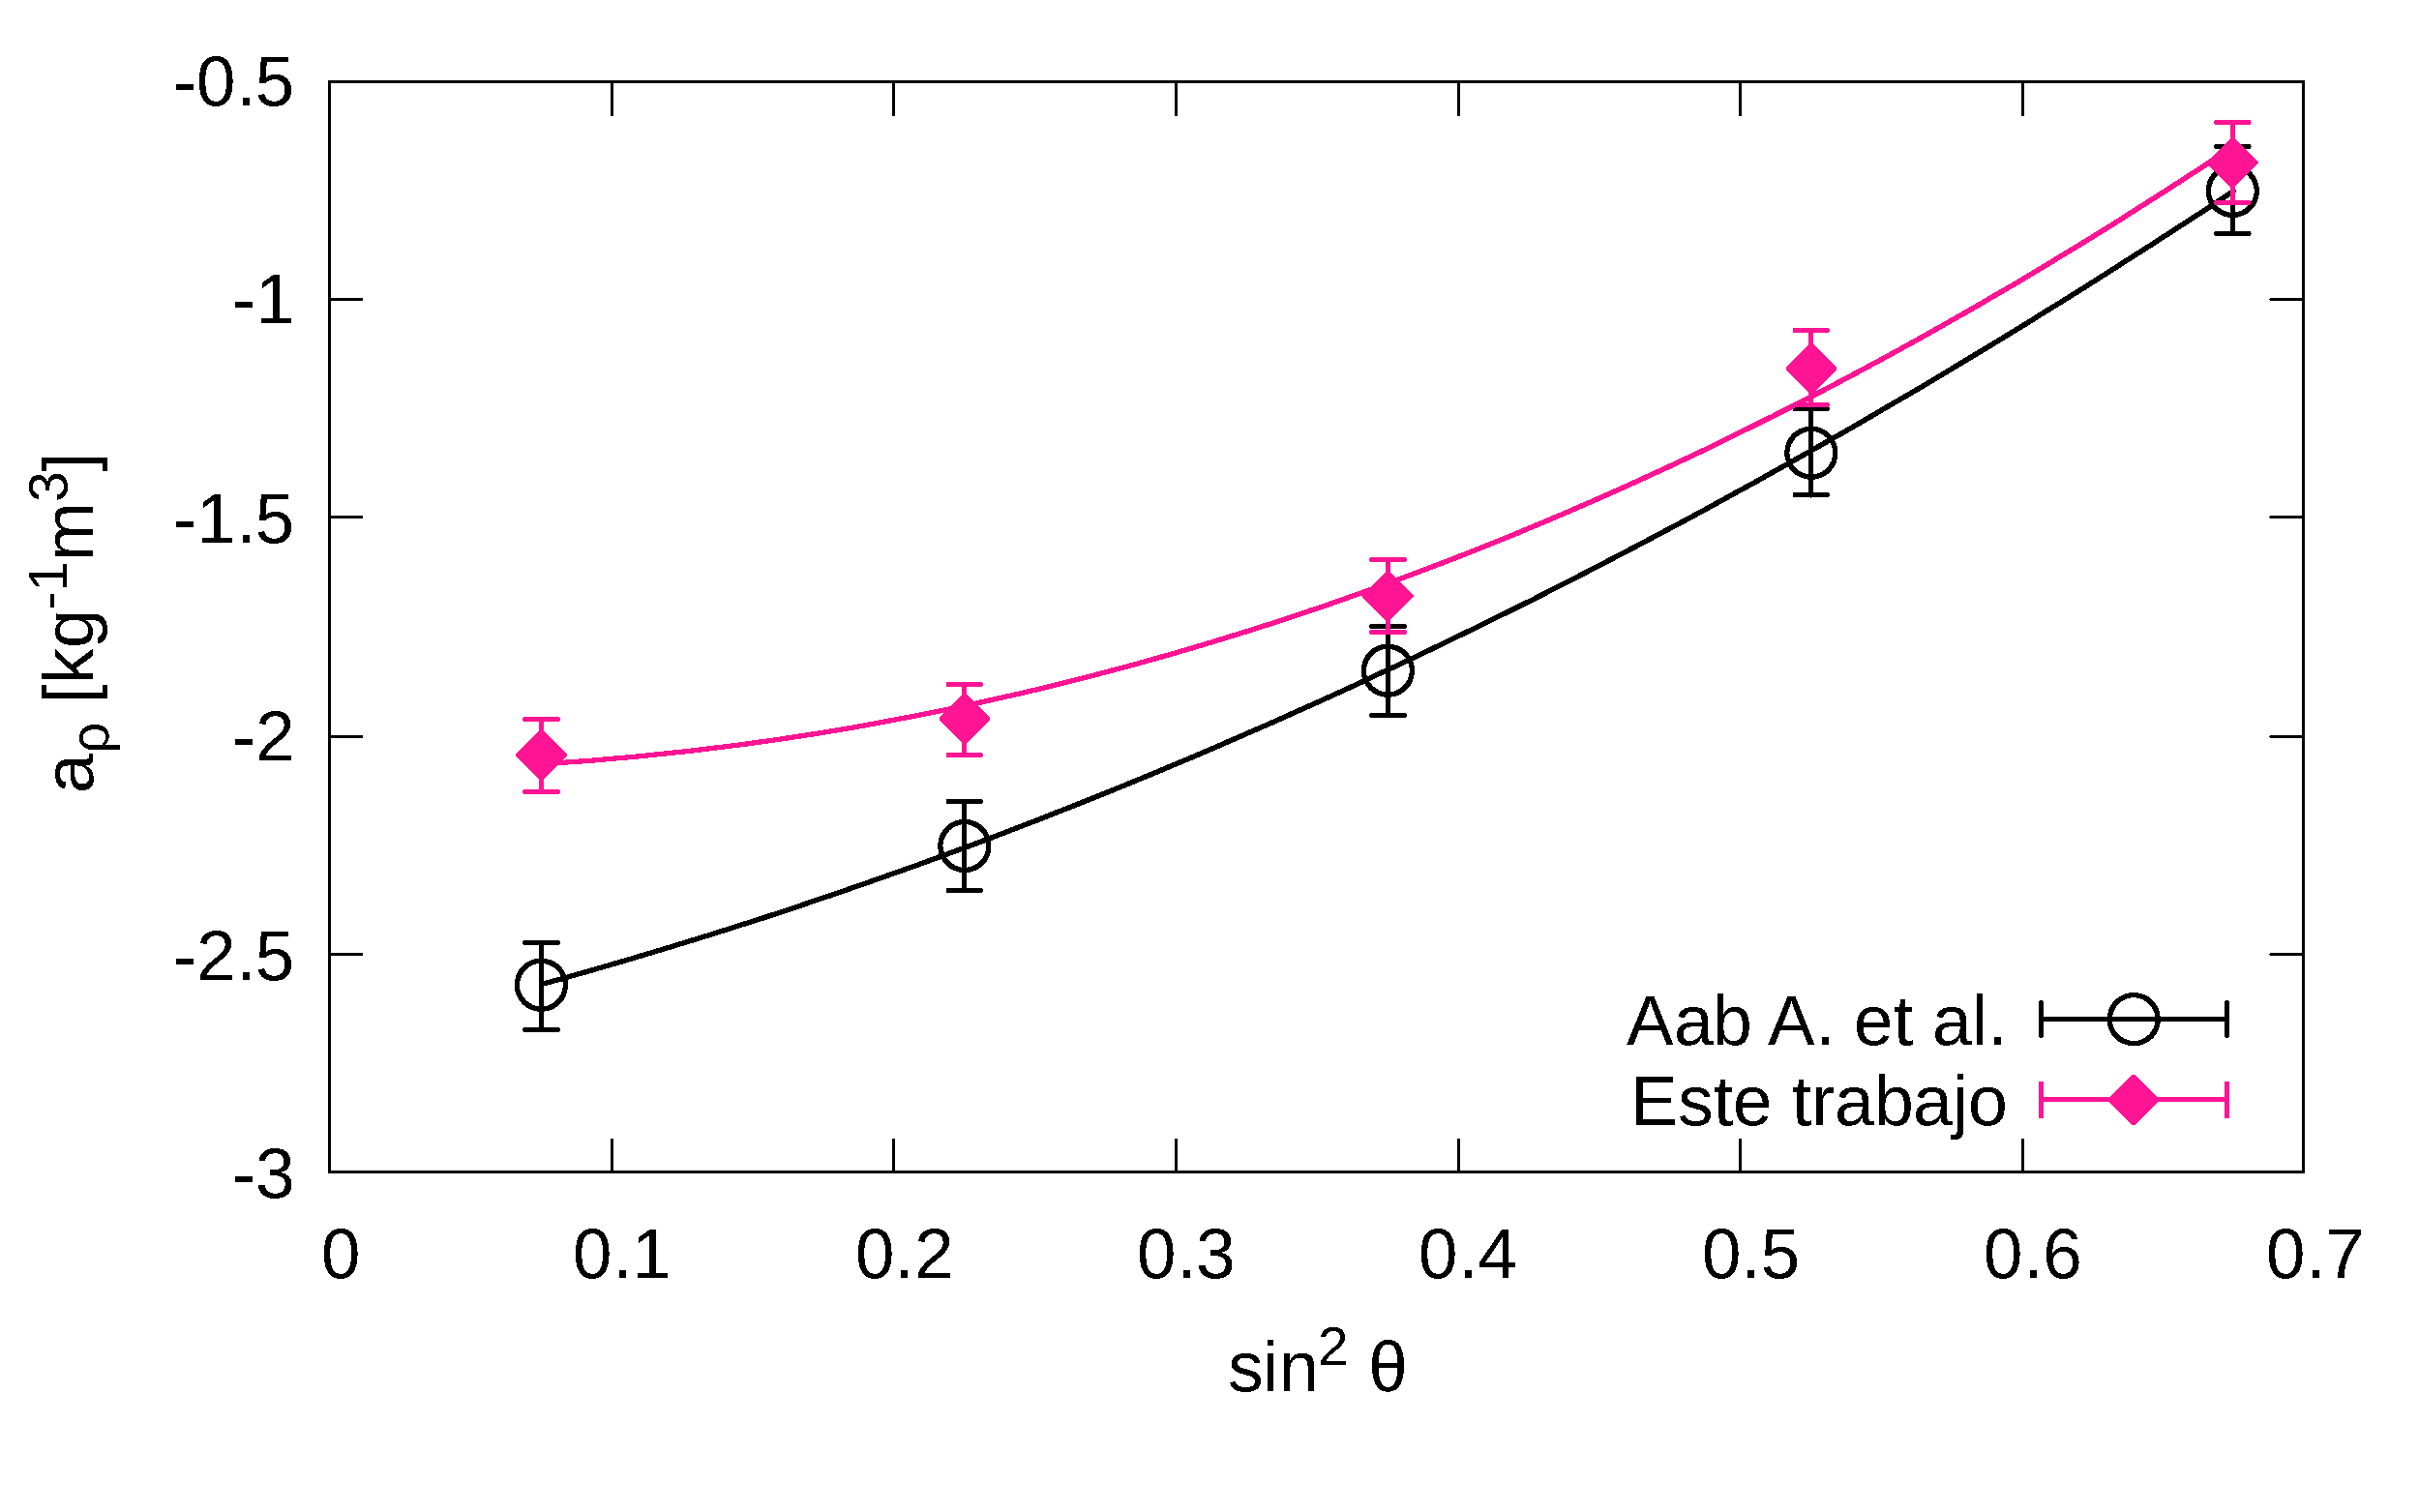
\includegraphics[width=0.5\textwidth]{arho.pdf}
        \end{center}
        \caption{}
        \label{fig:}
    \end{small}
\end{figure}


\begin{figure}[H]
    \begin{small}
        \begin{center}
            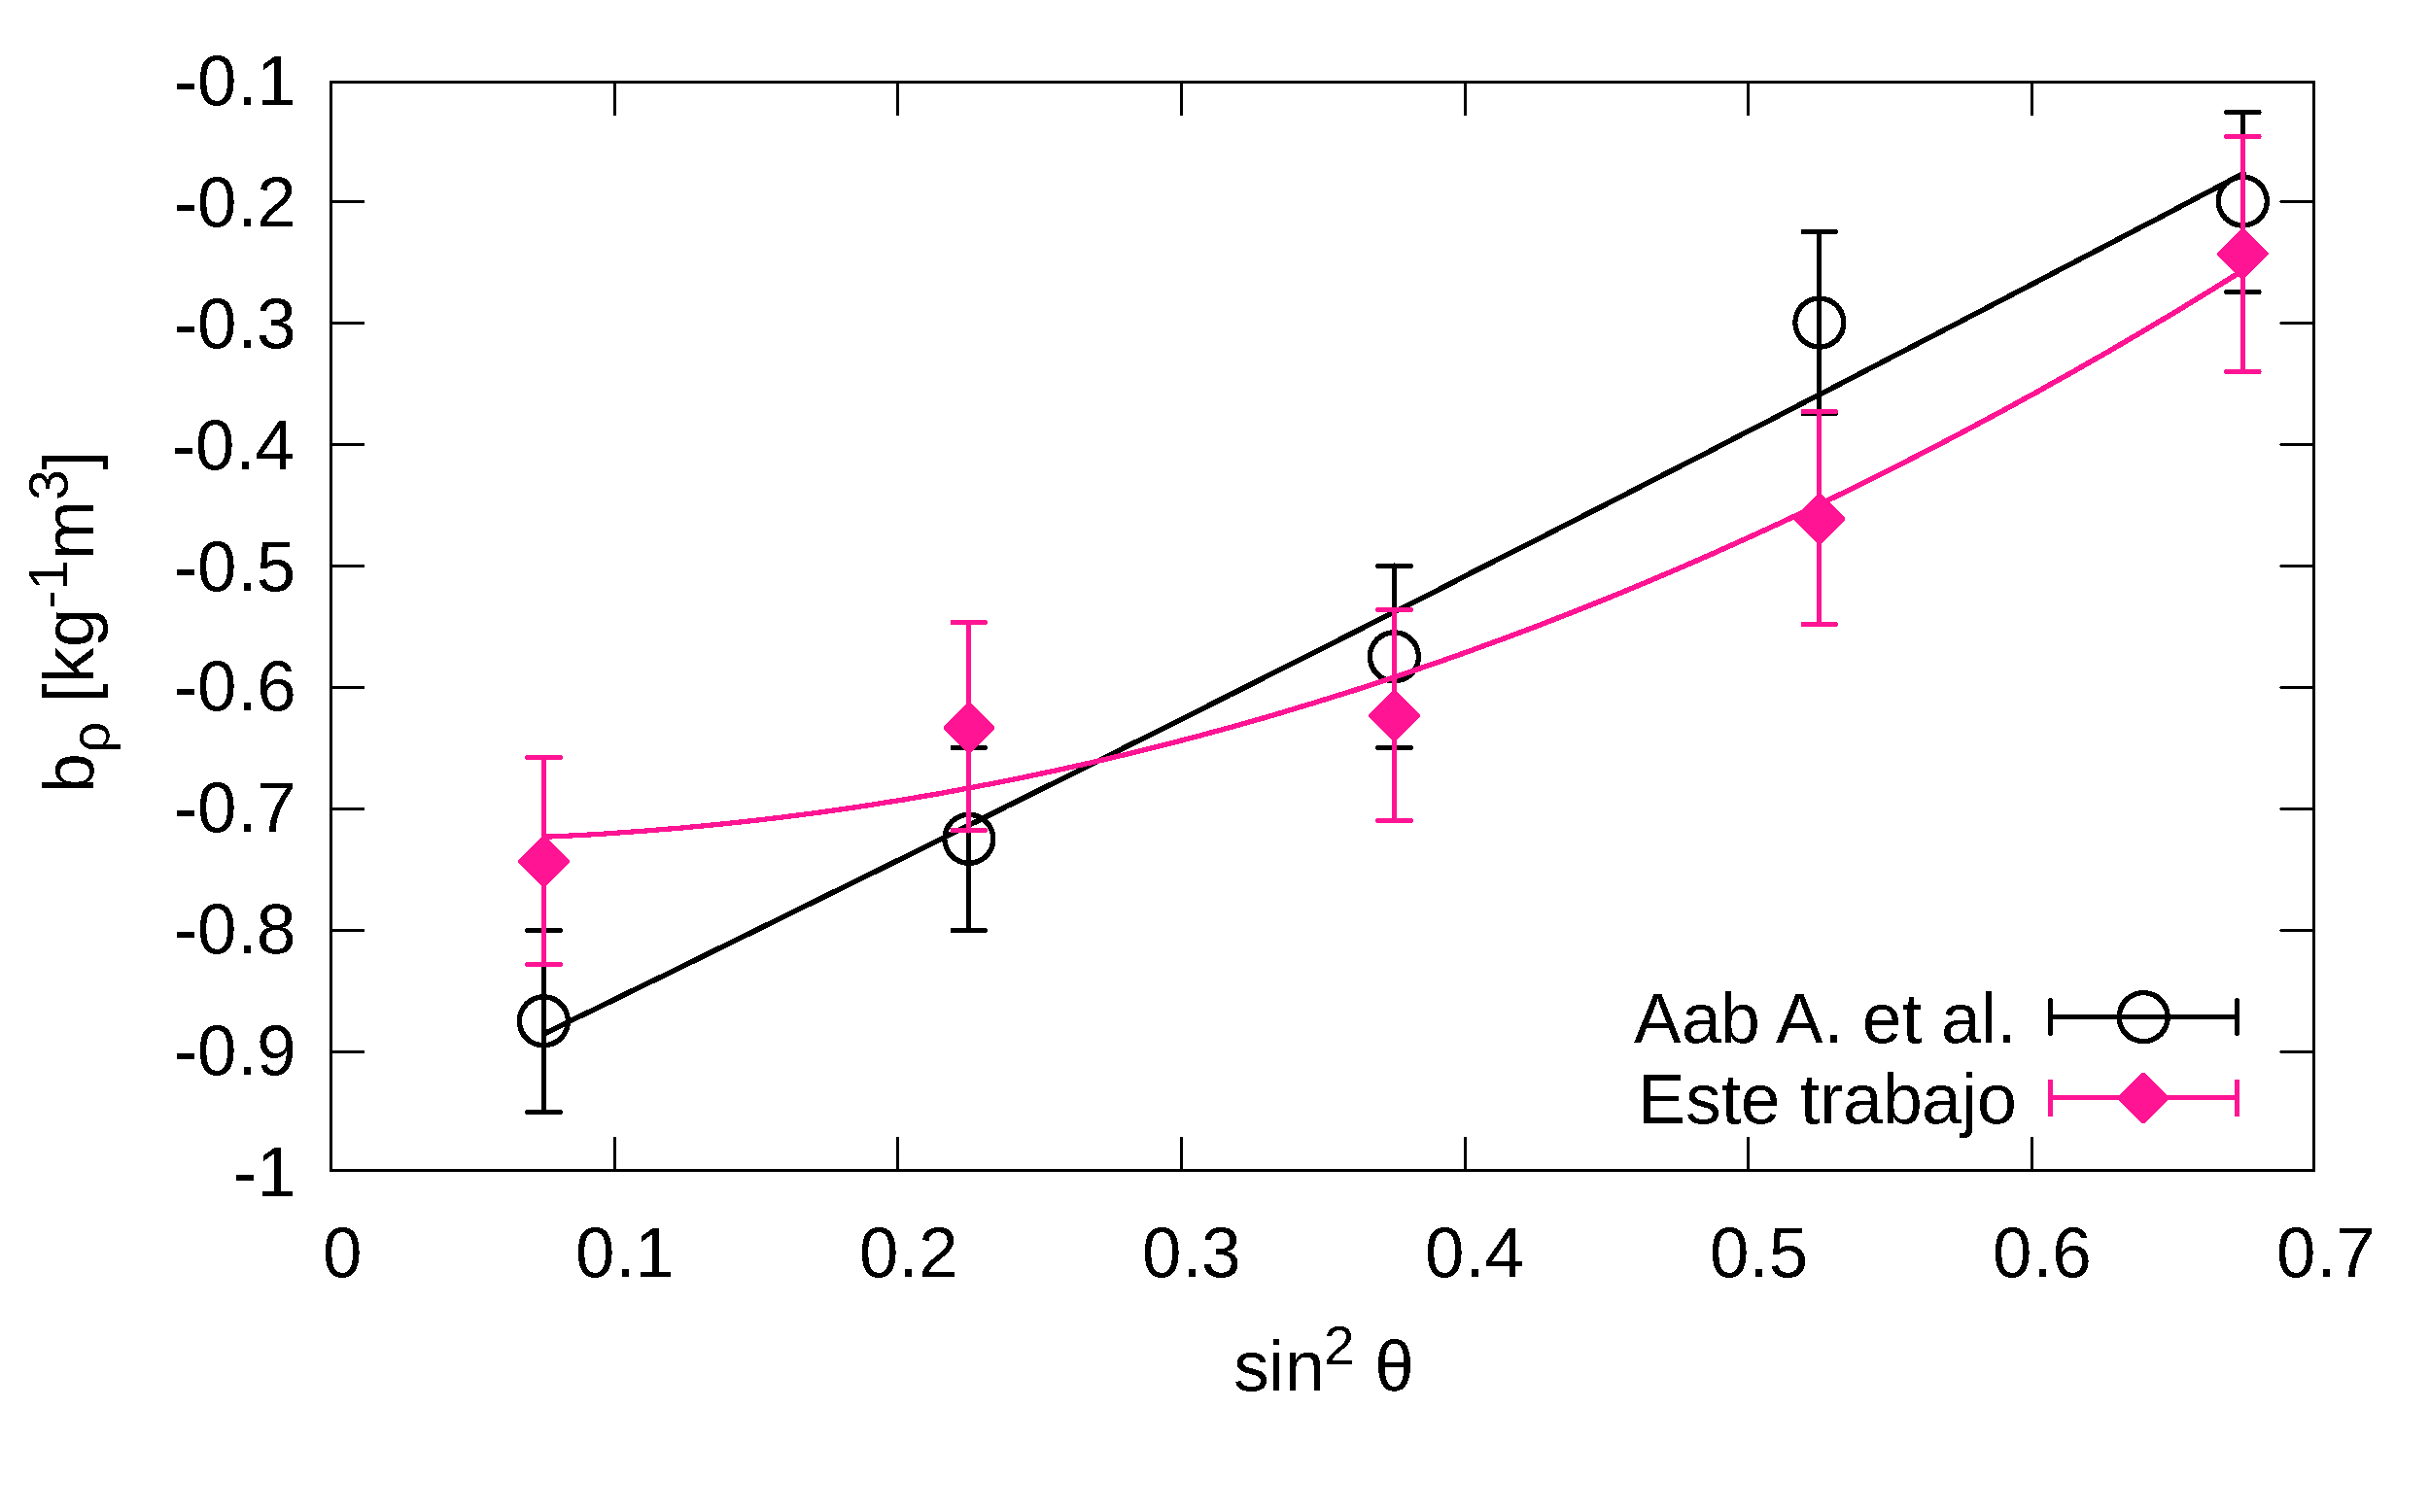
\includegraphics[width=0.5\textwidth]{brho.pdf}
        \end{center}
        \caption{}
        \label{fig:}
    \end{small}
\end{figure}


Para tener una idea si el modelo se ajusta a  lo observado experimentalmente, se consideran estos parámetros del clima independientes de $\theta$ y la tasa de eventos diaria, se obtiene el ajuste de la Fig.\ref{fig:tasa}. La media oscila alrededor  de $0.25$ eventos por $km^2$ por día, $\sim 56\%$ de aumento con respecto a la  media de eventos para el \emph{disparo estándar}.


\begin{figure}[H]
    \begin{small}
        \begin{center}
            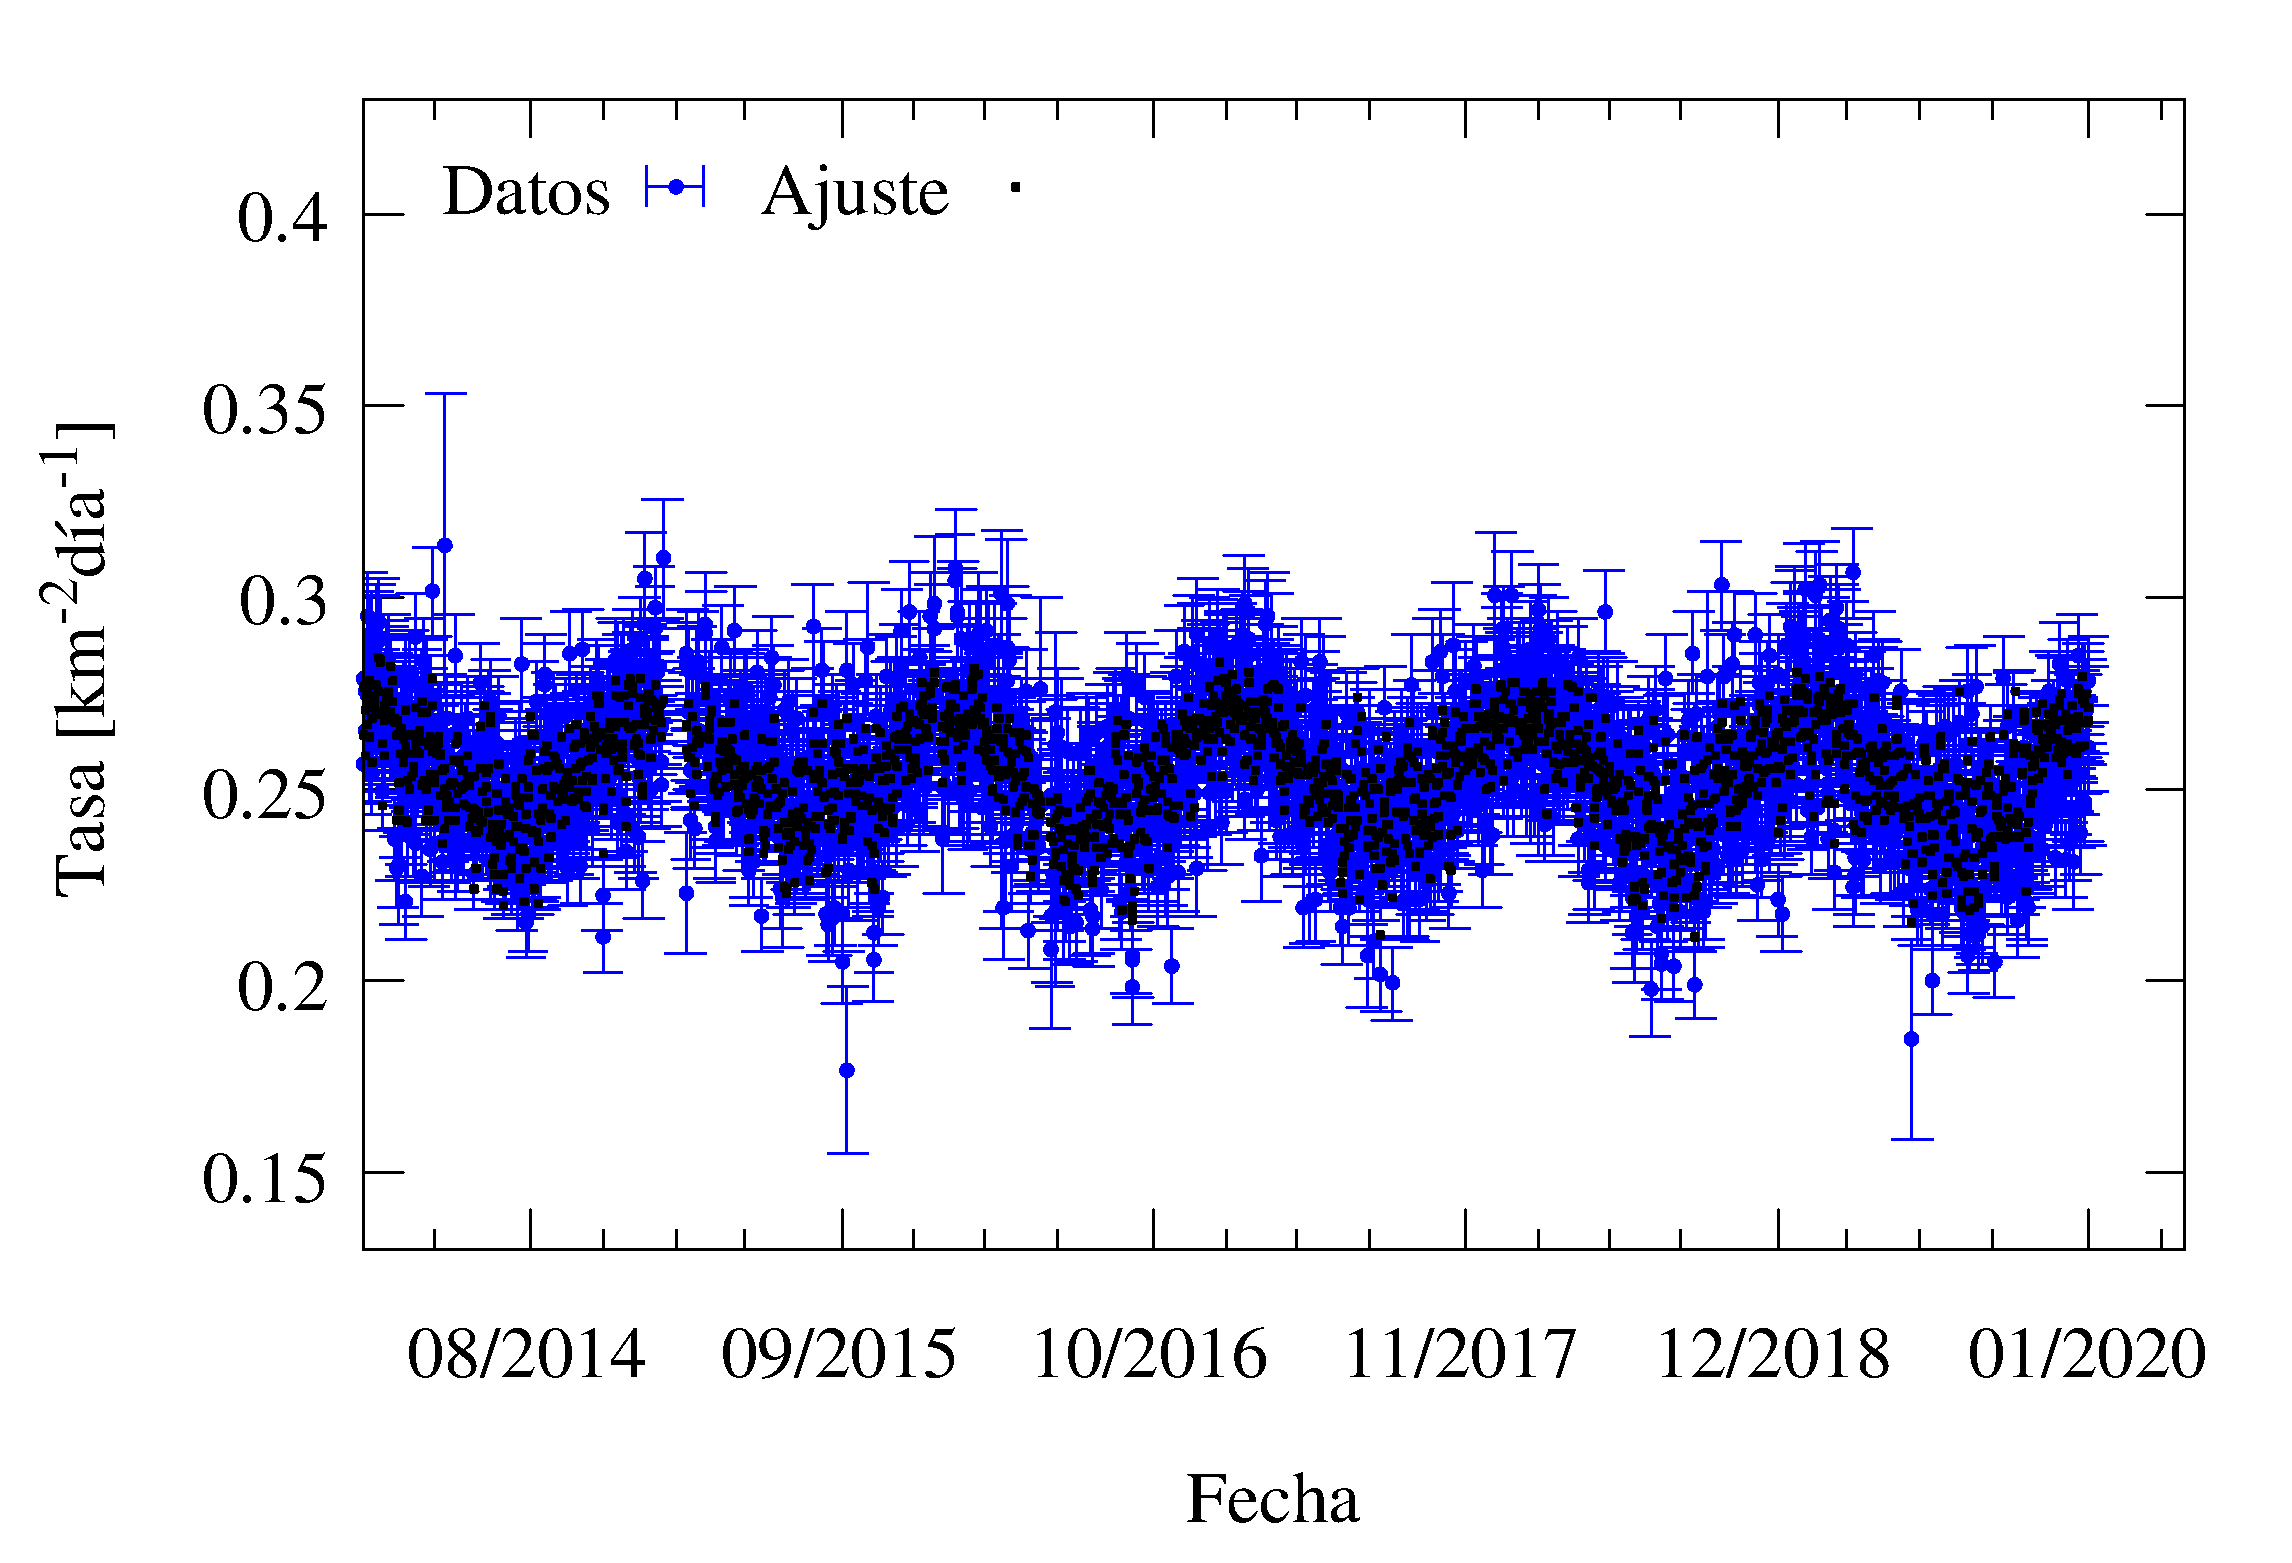
\includegraphics[width=0.5\textwidth]{rate_daily.pdf}
        \end{center}
        \caption{}
        \label{fig:tasa}
    \end{small}
\end{figure}

Si hacemos un promedio de la tasa por cada hora durante los años 2014 al 2019, se obtiene la figura \ref{fig:hora}.

\begin{figure}[H]
    \begin{small}
        \begin{center}
            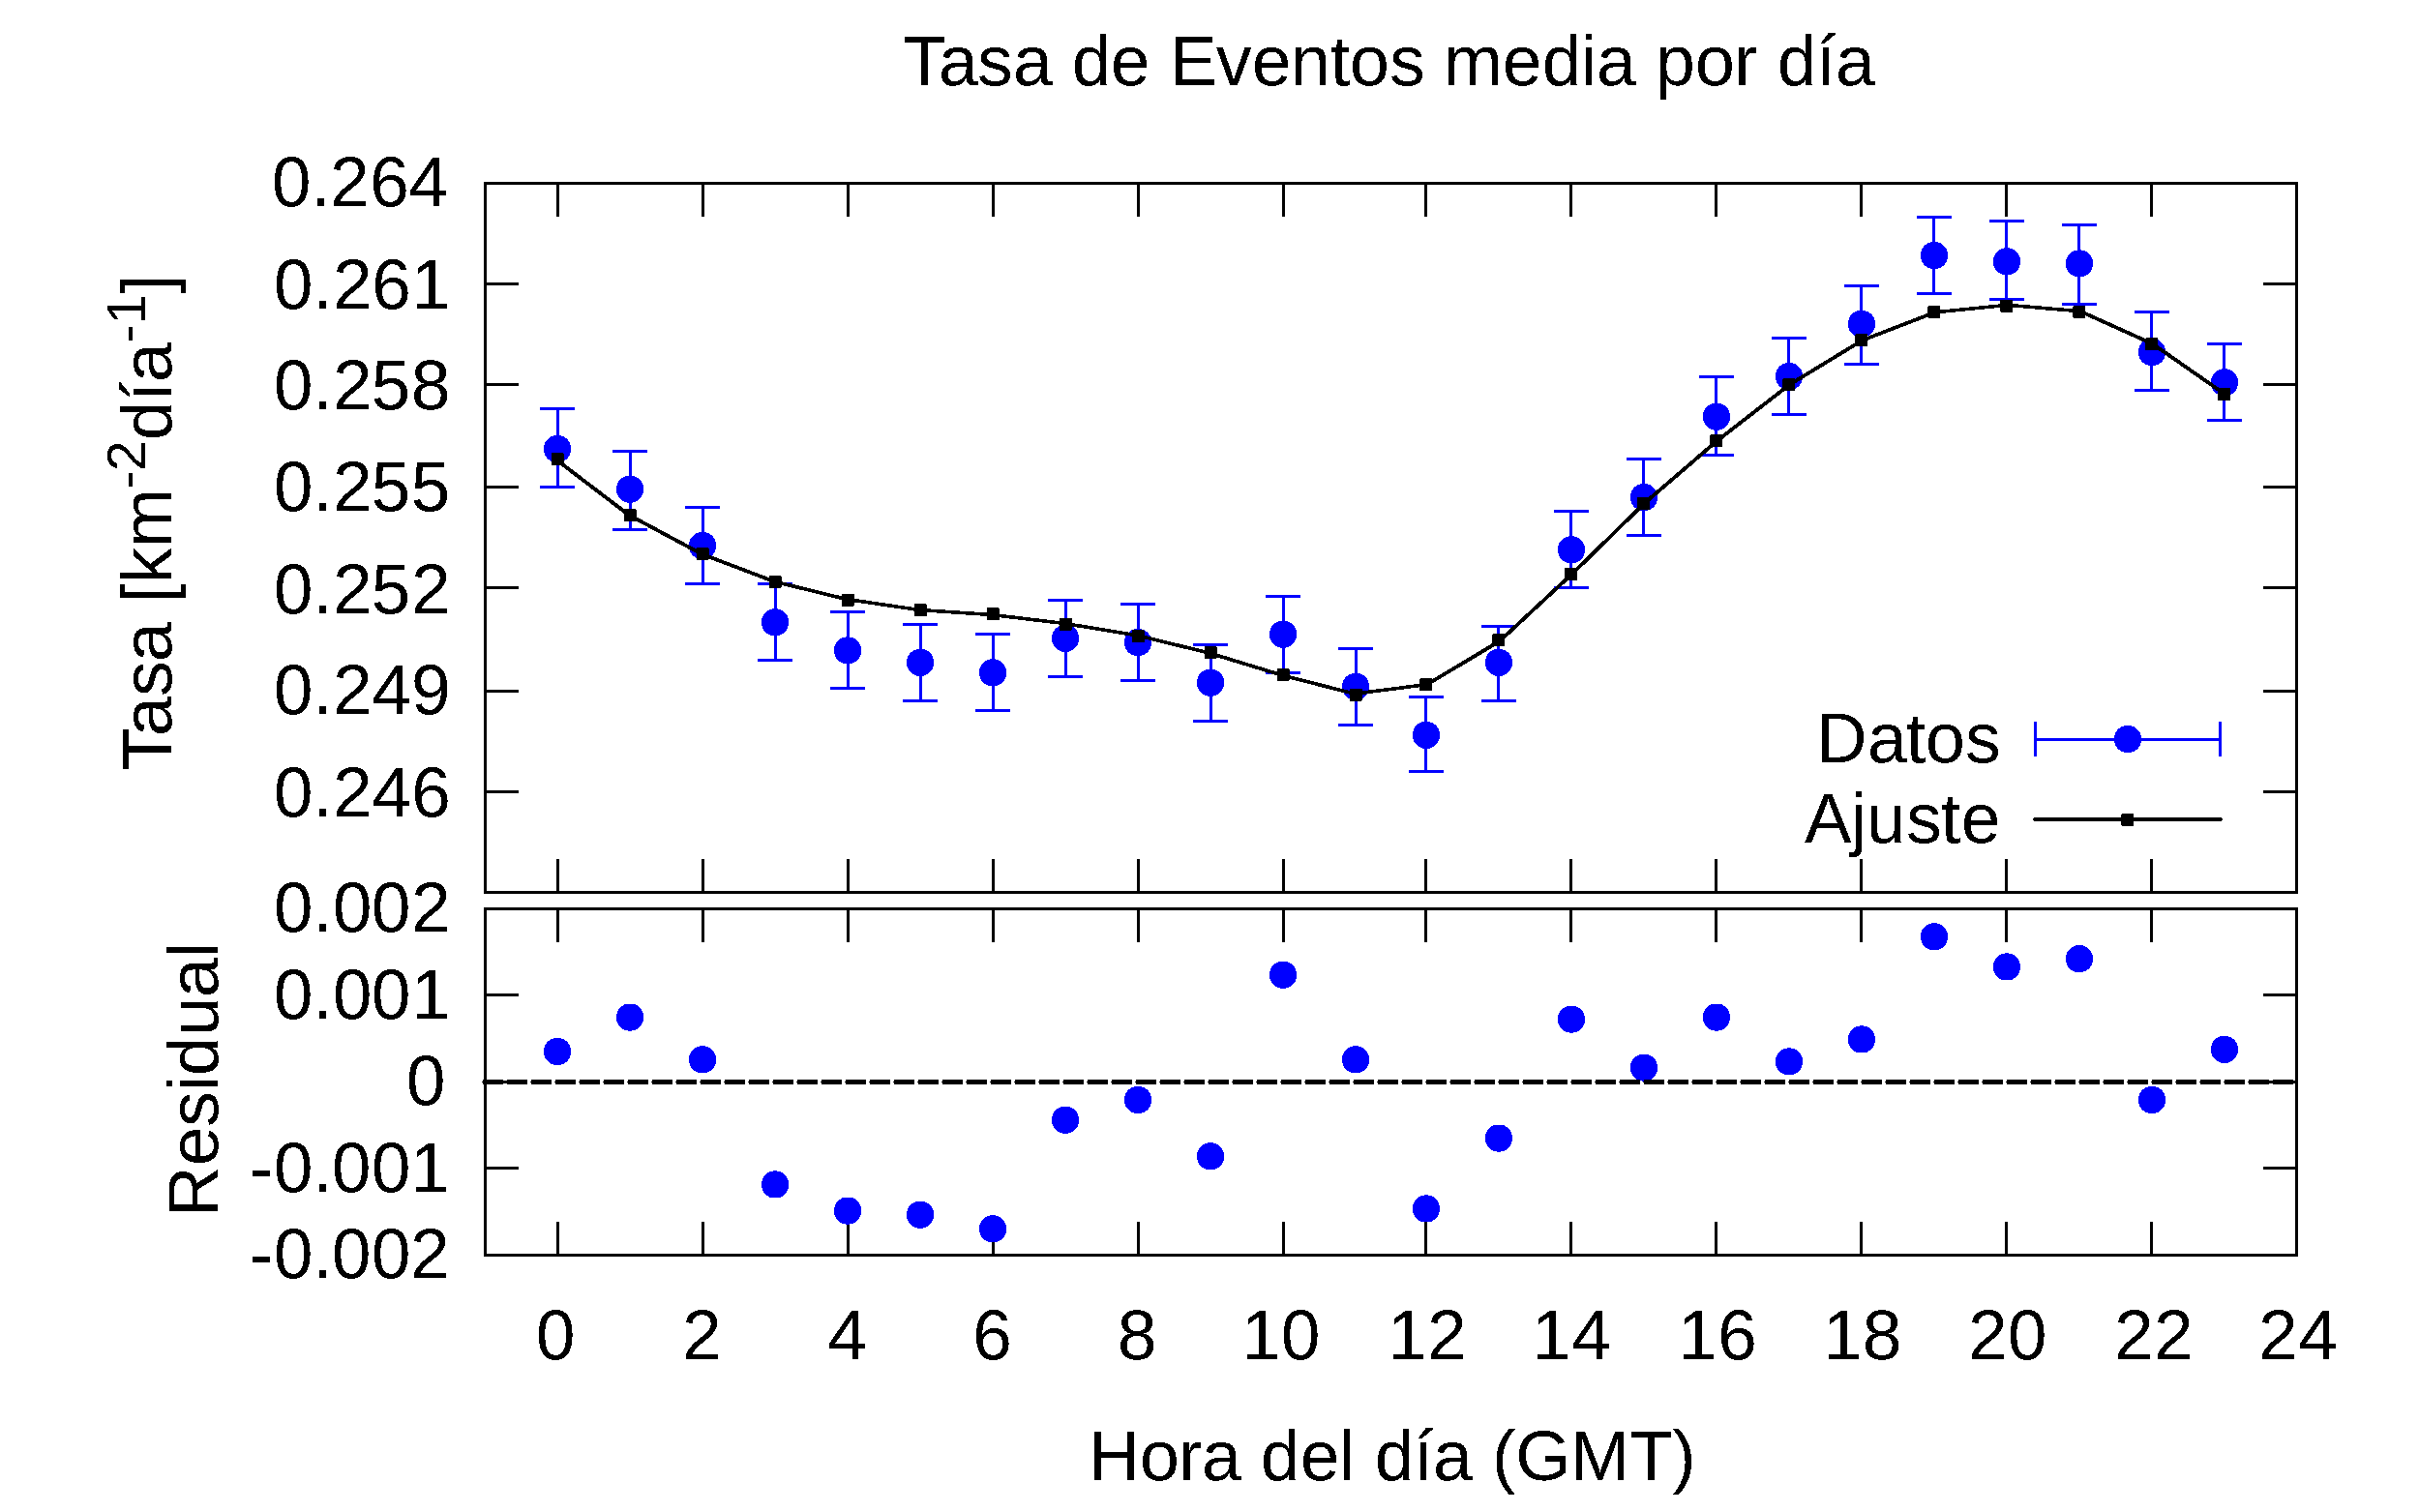
\includegraphics[width=0.5\textwidth]{rate_hourly.pdf}
        \end{center}
        \caption{}
        \label{fig:hora}
    \end{small}
\end{figure}


\section*{Corrección del clima}

En la Fig.\ref{fig:label} se muestra en `Referencia'(en azul) tiene la corrección del clima con los parámetros de la colaboración obtenidos en el 2017, que además son utilizados por el disparo estándar. En cambio la línea `Actual', que es corregida con los parámetros  obtenidos con datos de All Triggers, como se muestra en la sección anterior. 

Para obtener los resultados de la línea `Actual' del Fig.\ref{fig:label} seguí los siguientes pasos.

\begin{enumerate}
\item Cuando preparo el archivo para la corrección, me aseguro de que se esté imprimiendo el valor de $S_{38}$ sin corregir.
\item Para obtener la señal $S_0$, que en este caso $S_{38,0}$, uso la expresión $S_{38,0} = S_{38}/(1 + \alpha_P..+ ...) = S_{38,w}\times \frac{S(1000)}{S(1000)_w (1 + \alpha_P..+ ...)  }$  
\item Con este valor $S_{38,0}$ reconstruyo la energía con $E=A (S)^B$. Los parámetros A y B los obtuve de hacer el ajuste entre energía y S38 corregido por la colaboración. 
\item Me restrinjo a los eventos entre 1 - 2 EeV según la energía nueva.
\item Hago el análisis en el mismo rango de tiempo en el que analicé la línea de `Referencia'. 
\end{enumerate}


\begin{figure}[H]
    \begin{small}
        \begin{center}
            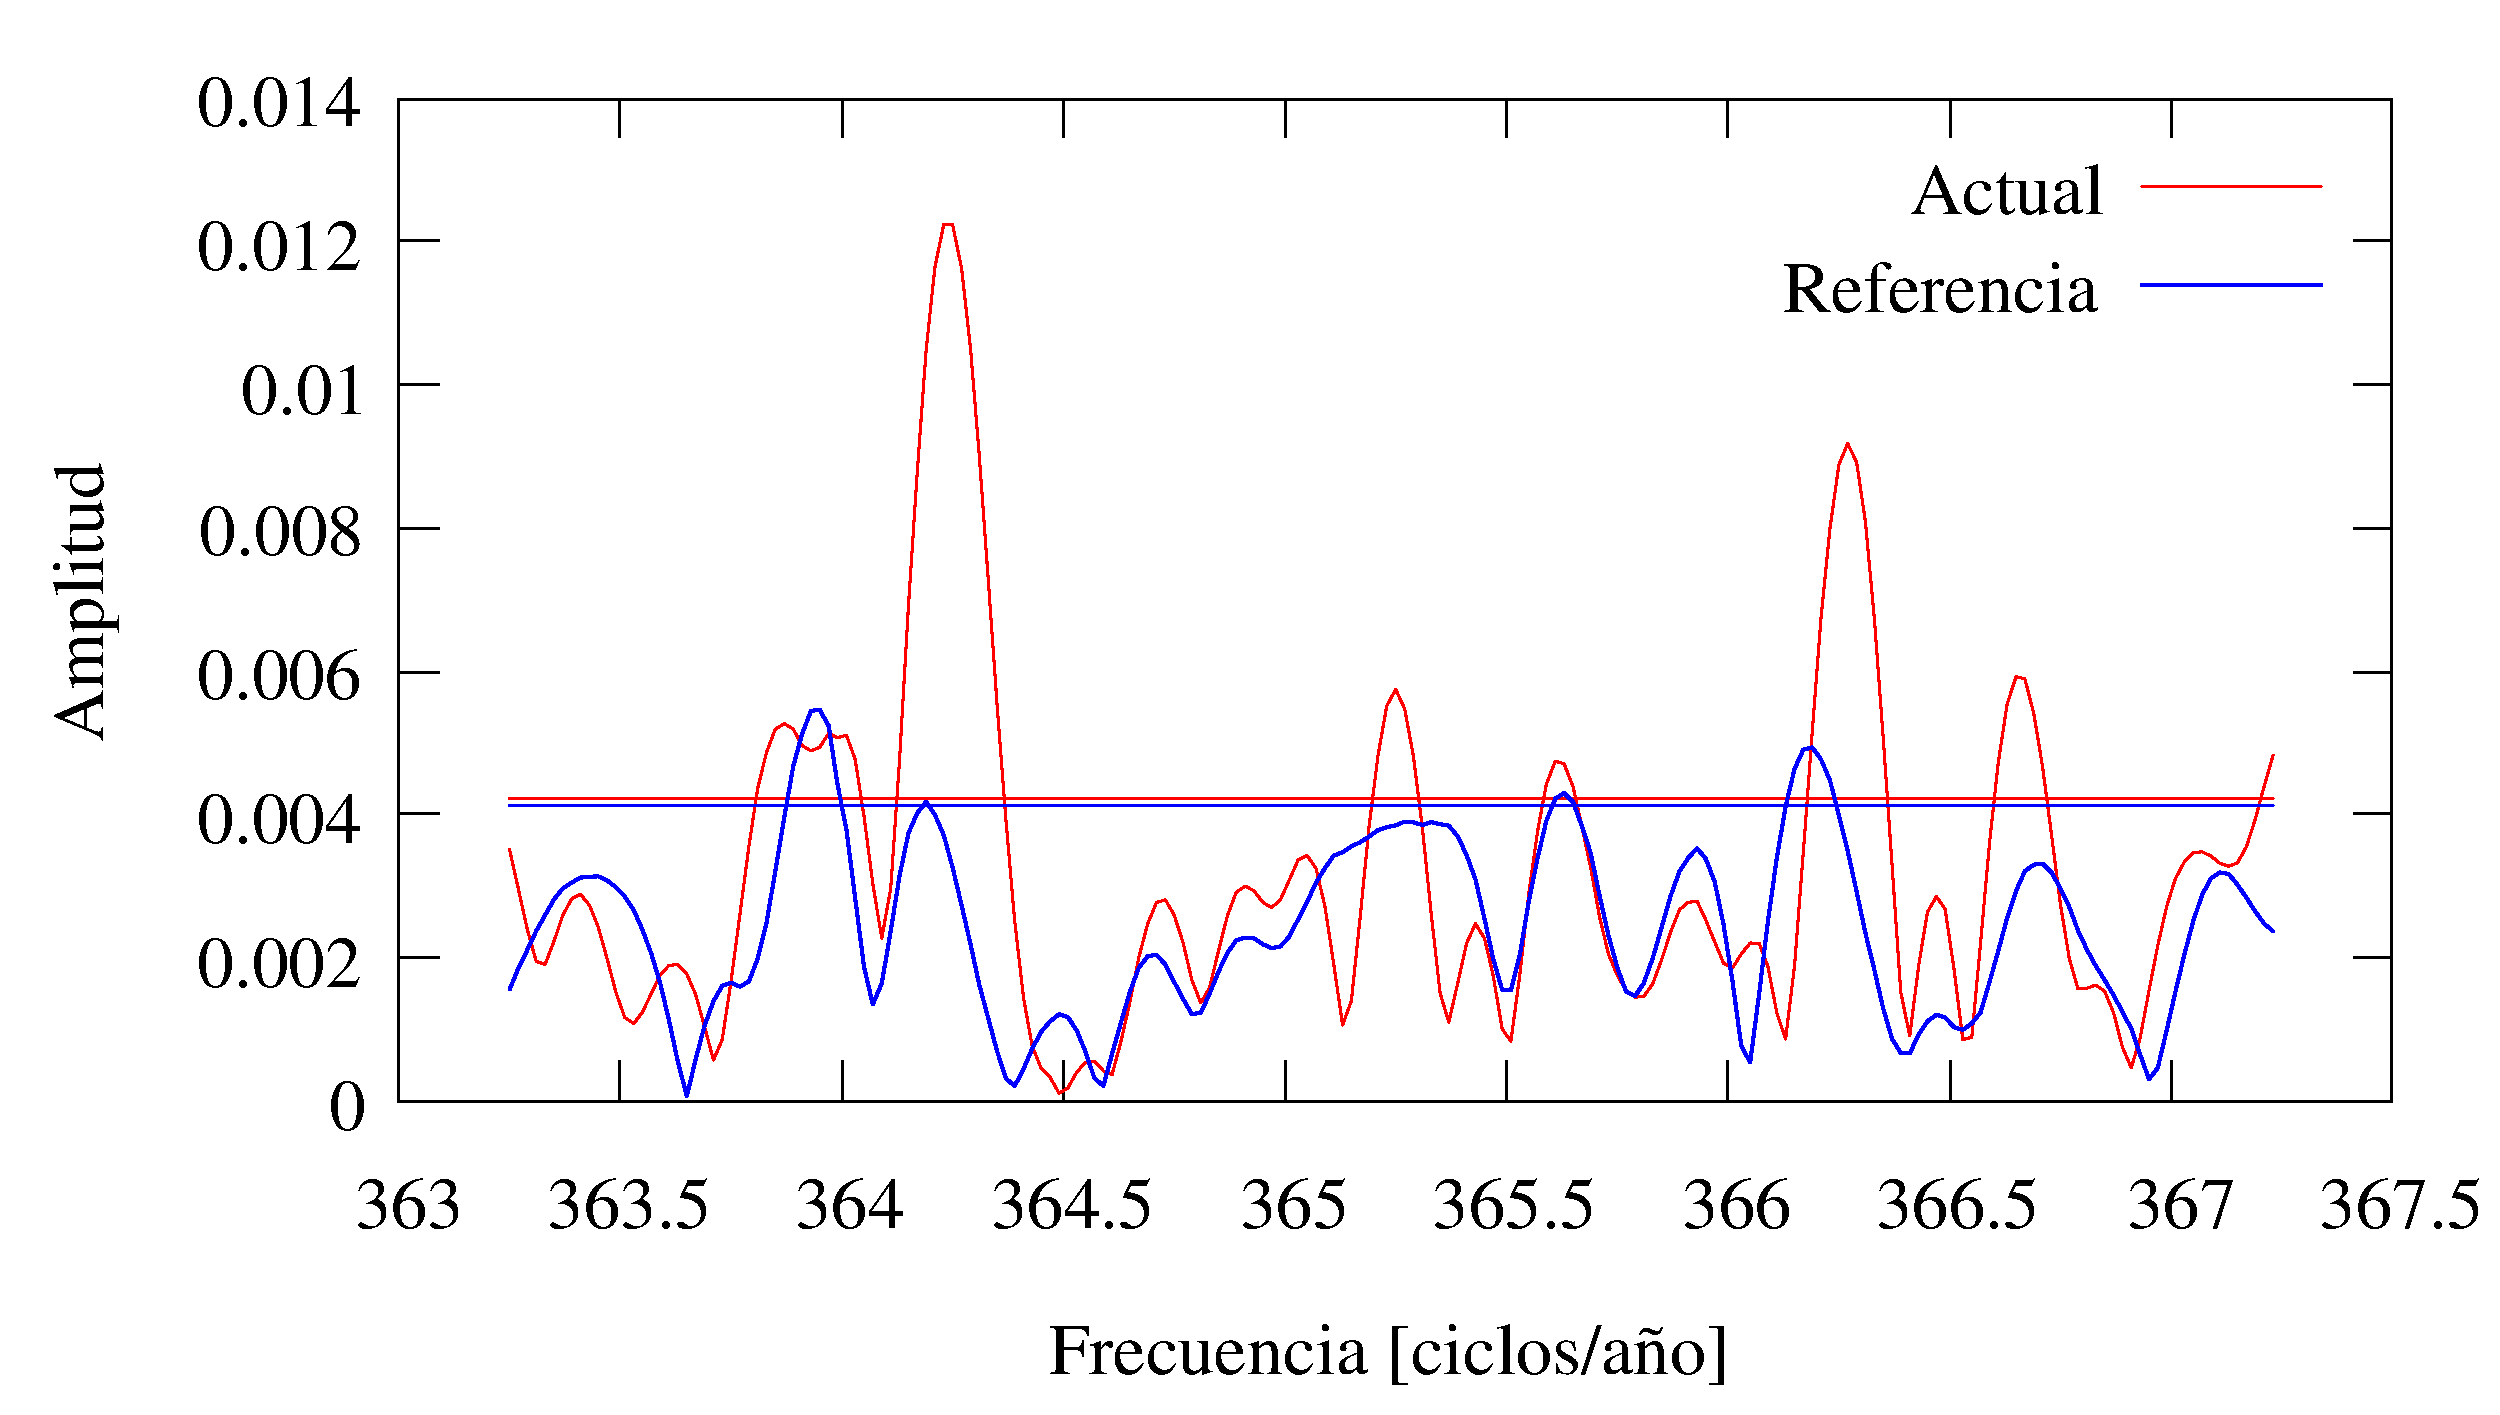
\includegraphics[width=0.5\textwidth]{anisotropia.pdf}
        \end{center}
        \caption{}
        \label{fig:label}
    \end{small}
\end{figure}

\end{document}